\documentclass[../main.tex]{subfiles}
\graphicspath{{img},{img/ink},{ink}}

\begin{document}

\begin{tcolorbox}[
    width=\textwidth,
    height=\textheight,
    title=Phyphox: Salatschleuder,
    fonttitle=\Large,
    before title=\vspace{0.2cm}, after title=\vspace{0.2cm},
    colback=white,
    title filled=true, 
    colbacktitle=myorange,
    colframe=black,
    coltitle=black,
    ]



    \begin{minipage}[]{0.5\textwidth}
        \vspace{0.2cm}
        \textbf{Klassenstufe}: 9/10

        \vspace{0.7cm}
        \textbf{Fachlicher Bezug}: Zentripetalbeschleunigung, Regressionsgerade
        
        \vspace{0.7cm} 
        \textbf{Material}:
        \begin{itemize}[noitemsep]
            \item Salatschleuder
            \item Stofftuch (T-Shirt, Handtuch, ...)
            \item Handy + Phyphox
        \end{itemize}
    \end{minipage}
    \hspace{1.8cm}
    \begin{minipage}[]{0.35\textwidth}
        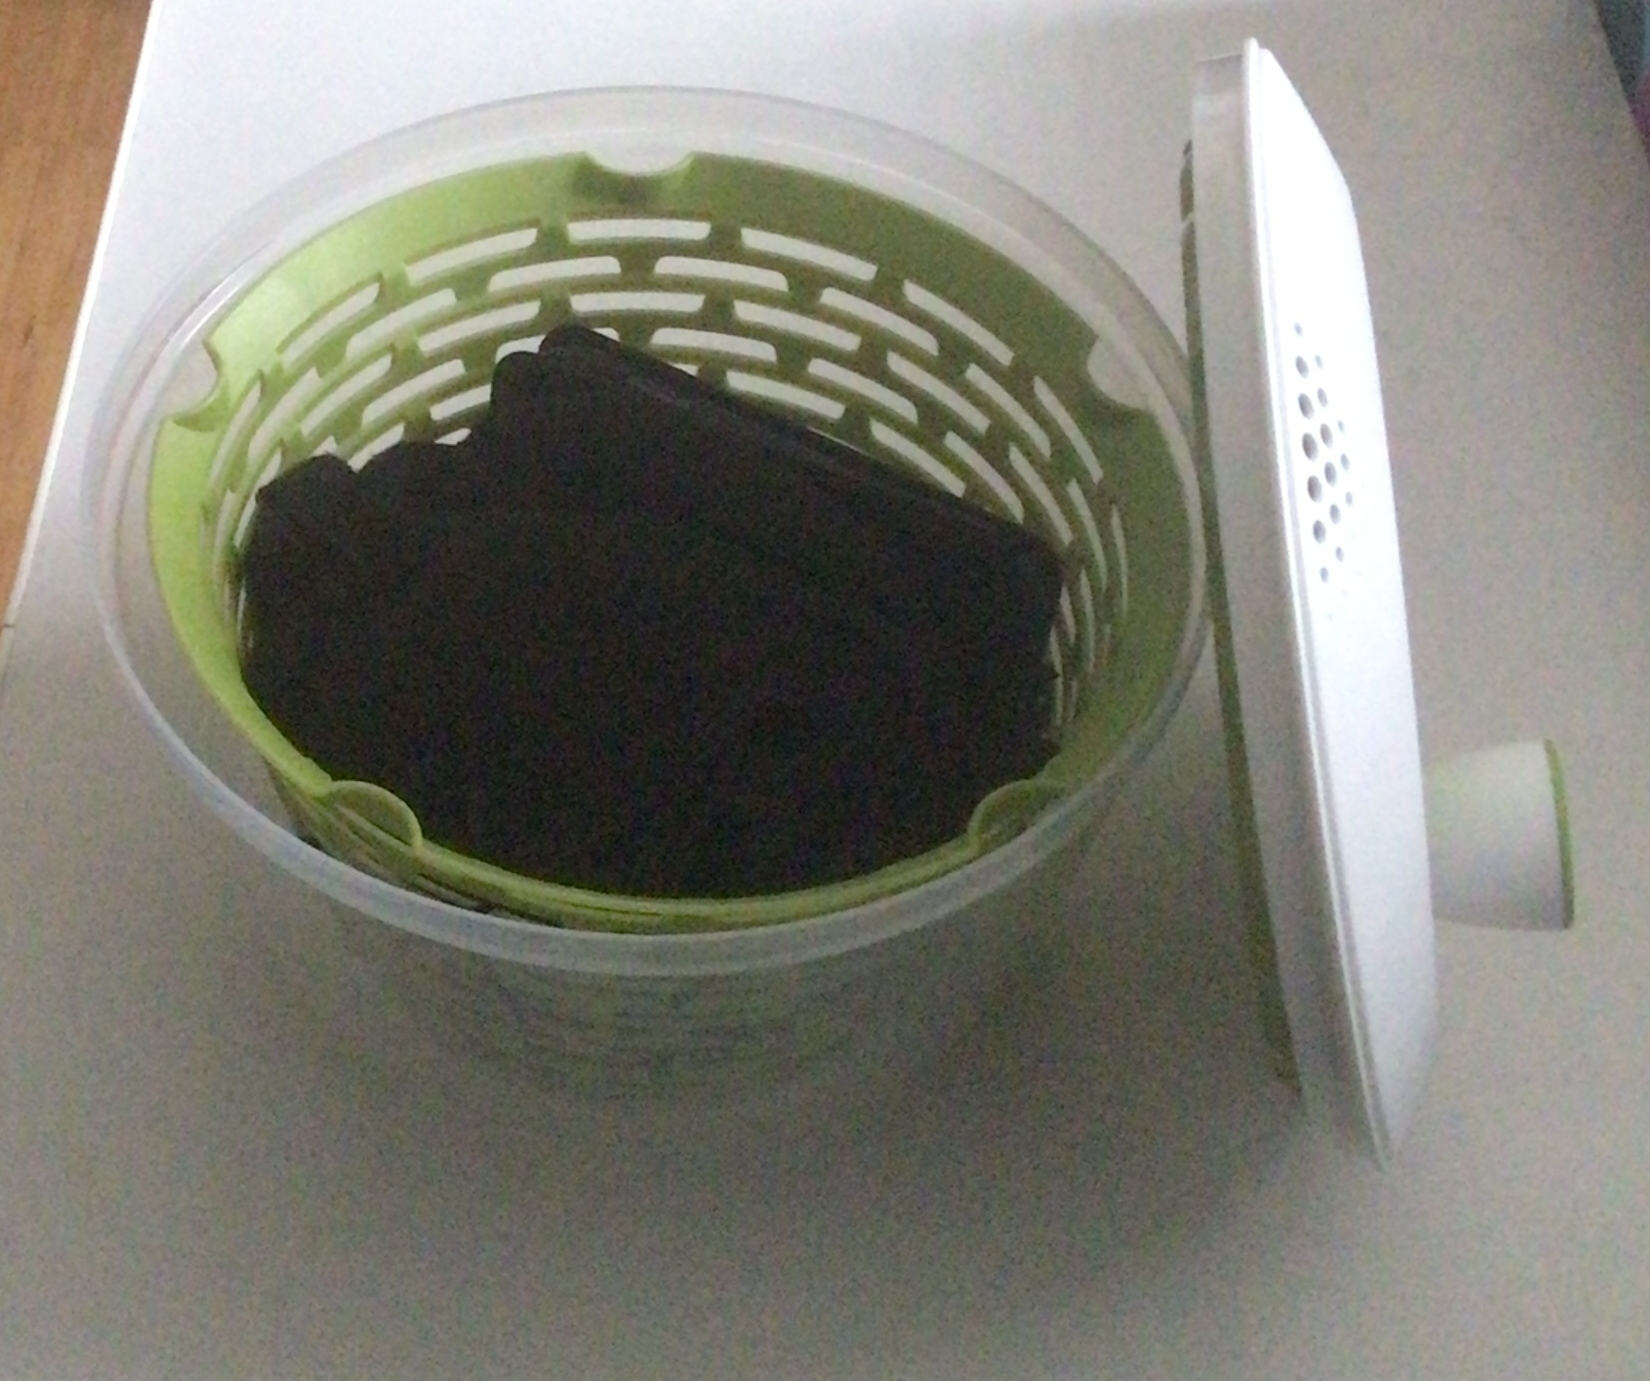
\includegraphics[width=\textwidth]{img/versuchsaufbau}
    \end{minipage}

    \vspace{0.7cm}
    \begin{minipage}[]{0.73\textwidth}
        \textbf{Aufbau}: Das Handy wird möglichst weit außen in der Salatschleuder platziert. Mit einem Stofftuch wird der Rest der Salatschüssel ausgefüllt, um dem Handy die notwendige Stabilität bei geringer Rotation zu geben.

        \vspace{0.7cm}
        \textbf{Durchführung}: In der Phyphox-App wird unter dem Reiter \glqq Mechanik\grqq{} die Auswahl \glqq Zentripetalbeschleunigung\grqq{} getroffen. Der Fernzugriff wird aktiviert. Über einen längeren Zeitraum wird versucht, möglichst viele Winkelgeschwindigkeiten zu duchlaufen. Das kann rein zufällig erfolgen.

        \vspace{0.7cm}
        \textbf{Ergebnis}: Im oberen Graph wird der Betrag der Beschleunigung $a$ gegen die Winkelgeschwindigkeit $\omega$ aufgetragen. Hier beobachtet man eine quadratische Abhängigkeit, also
        \begin{align*}
            a \sim \omega^2
        \end{align*}
        Wird dann im unteren Graph die Beschleunigung $a$ gegen das Quadrat der Winkelgeschwindigkeite $\omega^2$ aufgetragen, erhält man eine Gerade und die Steigung (Zoom $\rightarrow$ Mehr Werkzeuge) liefert den Proportionalitätsfaktor. Dieser ist gerade der radiale Abstand $R$ des Beschleunigungssensors zum Drehpunkt. 
        \begin{align*}
            a = R \cdot \omega^2
        \end{align*}
    \end{minipage}
    \hspace{0.2cm}
    \begin{minipage}[]{0.22\textwidth}
        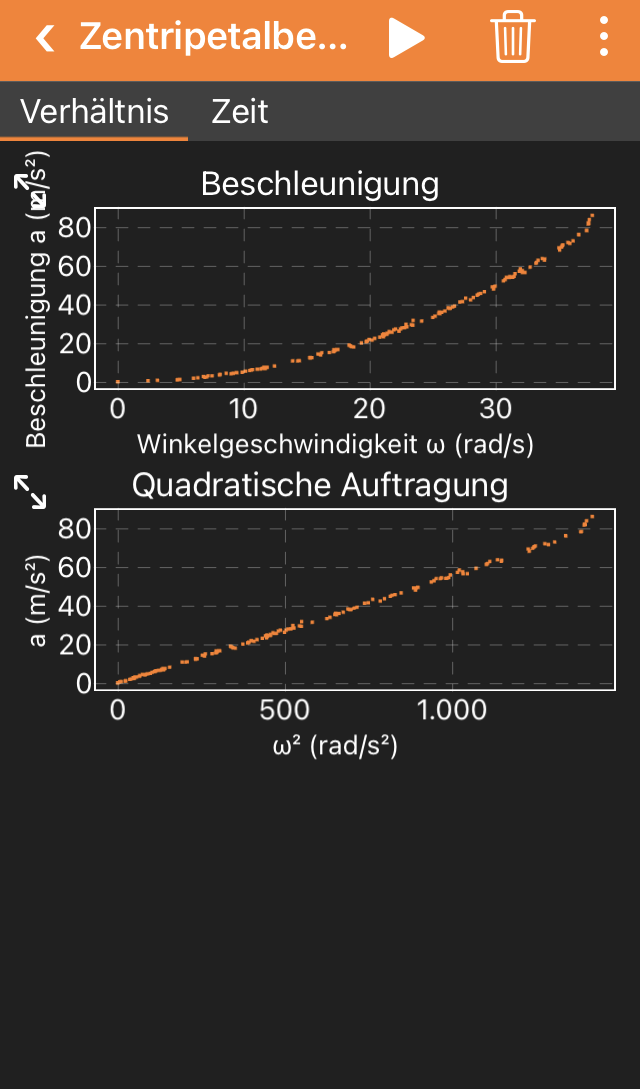
\includegraphics[width=\textwidth]{img/app1}

        \vspace{0.3cm}
        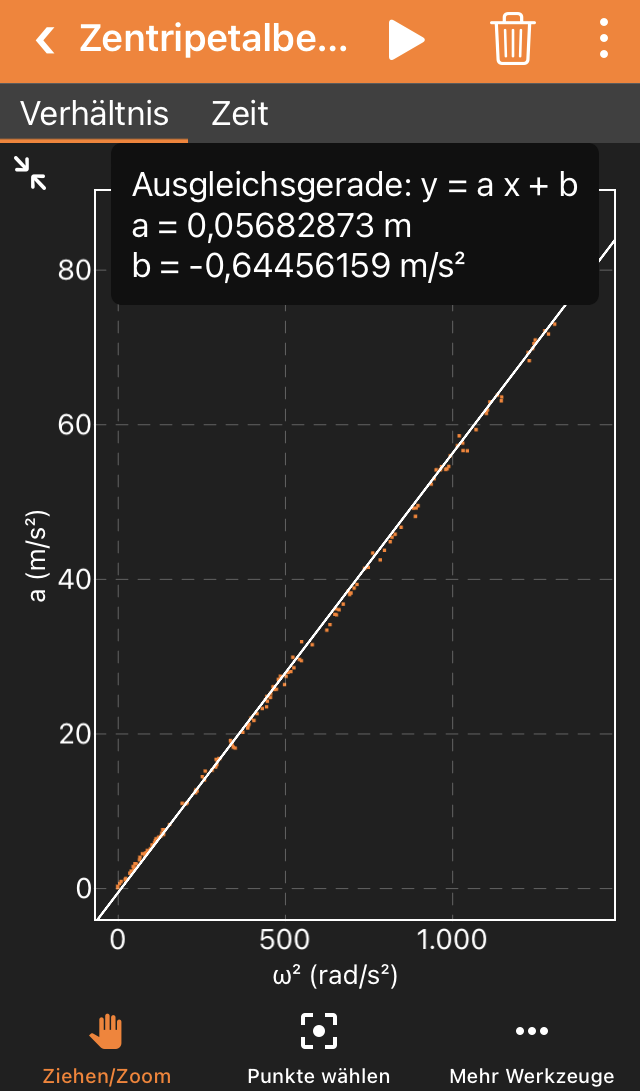
\includegraphics[width=\textwidth]{img/app2}
    \end{minipage}

    \vspace{0.7cm}
    \begin{minipage}[]{0.80\textwidth}
        \textbf{Bemerkung}: Besteht zusätzlich die Möglichkeit Drehbewegungen mit unterschiedlichem Radius $R$ zu untersuchen, kann ein eigenes Experiment erstellt werden. Zur besseren Unterscheidung erhält jede Drehbewegung eine eigne Farbe.

    \end{minipage}
    \hspace{0.1cm}
    \begin{minipage}[]{0.15\textwidth}
        \vspace{0.5cm}
        
\includegraphics[width=\textwidth]{img/qr_code}
    \end{minipage}


\end{tcolorbox}


\end{document}
